% ----------------------------------------------------------
% Sumário
% ----------------------------------------------------------

\noindent\textbf{SUMÁRIO}\label{section:sumario}

% Por falta de tempo para fazer algo bem trabalhado, parte do sumário terá que ser manual mesmo. Podes observar como construi o sumário abaixo e utilizar como auxílio.

    \begin{enumerate}
        \item \textbf{Construção do Robô}
        \item \textbf{Criação de um ambiente no Gazebo}
        \item \textbf{Adição de funcionalidade}
        \item \textbf{Implementação de controle via teclado}
        \item \textbf{Integração completa com o ROS2}
        \item \textbf{conclusoes}
    \end{enumerate}

\hyperlink{referencias}{\textbf{REFERÊNCIAS}}

\vspace{0.3cm}
\hyperlink{apendices}{\textbf{APÊNDICES}}
% Caso tenham apêndices dentro da seção, essas duas linhas são retiradas do texto. Sendo assim, ficariam apenas as referências aos próprios apêndices (APÊNDICE A, APÊNDICE B, APÊNDICE C, etc...). Caso não tenha apêndices, retirar esse item do sumário.

\vspace{0.3cm}
\hyperlink{figuras}{\textbf{APÊNDICE A - FIGURAS}}

\vspace{0.3cm}
\hyperlink{tabelas}{\textbf{APÊNDICE B - TABELAS}}

\vspace{0.3cm}
\hyperlink{diagramas}{\textbf{APÊNDICE C - DIAGRAMAS}}

\vspace{0.3cm}
\hyperlink{anexos}{\textbf{ANEXOS}}

\vspace{0.3cm}

\hyperlink{despedida}{\textbf{ANEXO A - DESPEDIDA}}

\clearpage

% ----------------------------------------------------------
% ELEMENTOS TEXTUAIS
% ----------------------------------------------------------
%\vspace{0.5cm}

\gdef\clearforchapter{}
% ----------------------------------------------------------
% Introdução
% ----------------------------------------------------------

\chapter{Construção do Robô}\label{chapter:construcao}

Ao seguir o tutorial disponível nos sites do ROS2 e do Gazebo nós pudemos notar que o robô proposto a construir era bem similar ao apresentado em sala, e como tivemos problemas ao encontrar modelos de robôs que pertencessem ao \textit{Gazebo Fortress}, já que os modelos encontrados inicializavam na versão descontinuada do \textit{Gazebo}, decidimos manter um robô com o frame parecido ao original do tutorial, realizando apenas sutis diferenças. Na figura \ref{fig:URDF} podemos perceber que o site de referência de modelos de robôs indica que não é compatível com o \textit{ROS2 Humble}, pois apesar de ter modelos interessantes de serem simulados ainda estávamos procurando por modelos descritos em URDF.

\begin{figure}[h]
    \centering
    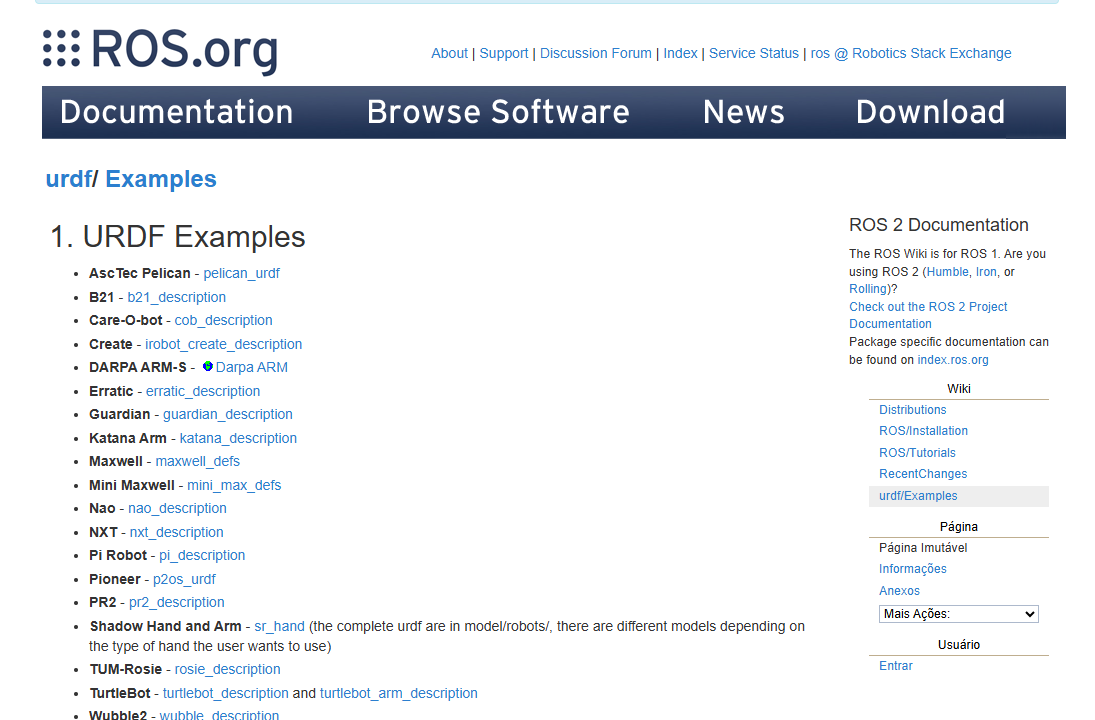
\includegraphics[width=0.5\linewidth]{Figuras/URDF.png}
    \caption{Modelos de Robo disponíveis em URDF}
    \label{fig:URDF}
\end{figure}

Durante a construção do robo alteramos os tamanhos da caixa e das rodas, além de mudar a cor para poder identificar e fazer alterações no documento sdf.







\vspace{0.5cm}
\chapter{Criação de um ambiente no Gazebo}\label{chapter: criacao}

Para poder testar os sensores a serem incluídos no robô nós incluímos objetos no mundo tanto manualmente como através da interface do ROS, podendo assim criar obstáculos que o robô pudesse identificar e desviar. A figura abaixo mostra como o mundo está configurado.

\begin{figure}[h]
    \centering
    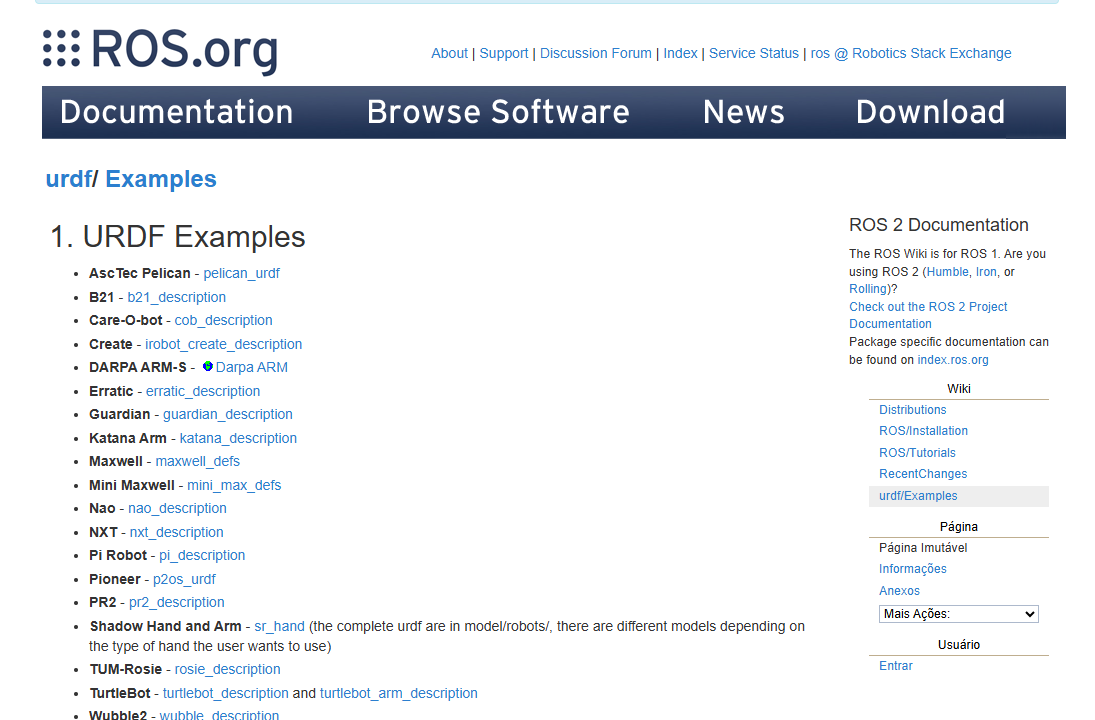
\includegraphics[width=0.5\linewidth]{Figuras/URDF.png}
    \caption{Modelos de Robo disponíveis em URDF}
    \label{fig:URDF}
\end{figure}


\chapter{Adição de funcionalidade}\label{Funcionalidades}

Como utilizamos o modelo disponibilizado em sala, nós já possuíamos 3 modelos de sensor em uso: sensor de contato que indica colisão, sensor IMU para medidas inerciais (giroscópio, acelerômetro e bússola magnética), e o lidar. Para poder adicionar mais sensores e incrementar o nosso robô decidimos adicionar um sensor \textit{GPS}, que no \textit{ROS2} é nomeado \textit{NAVSAT}, e uma câmera. Segue abaixo como ficou a nossa interface após configurar corretamente a câmera e o \textit{GPS}.



\chapter{Implementação de controle via teclado} \label{Implementação}


\chapter{Integração completa com o ROS2} \label{Integração}




% ----------------------------------------------------------
% Conclusões
% ----------------------------------------------------------

\vspace{0.5cm}
\chapter{CONCLUSÕES}\label{chapter:conclusoes}



% ----------------------------------------------------------
% Referências
% ----------------------------------------------------------
\vspace{0.5cm}
\noindent\hypertarget{referencias}{\textbf{REFERÊNCIAS}}
\addcontentsline{toc}{section}{Referencias}
\vspace{0.5cm}
\renewcommand{\refname}{ }
\renewcommand{\bibname}{ }
\vspace{-11mm}
\bibliography{Texto/referencias}

